\documentclass[9pt, handout=show,notes=show]{beamer}
\usetheme[width=0cm]{Goettingen}
\usecolortheme{rose}
\useoutertheme{default}

\usepackage{hyperref}
\usepackage{fontspec} 
\setsansfont{Futura LT} %%COMMENT ÇA SE LA RACCONTE!!


\usepackage{arydshln}
\usepackage{amsmath}
\usepackage{alltt}

\usepackage{mathptmx}
\usepackage{latexsym}
\usepackage{mathtools}
\usepackage{multirow}


\title{Brief summary of the past two month}
\date{21 Janvier 2016}

\begin{document}

\begin{frame}{ Winter Simulation Conference}
    A lot of\dots\\
    \includegraphics[width=5cm]{images/op.jpg}
    \includegraphics[width=5cm]{images/optimization.jpg}

    
\end{frame}

\begin{frame}{But..}
    \begin{itemize}
	\item random interesting stuff (reflection around $p-values$, philosophical issues, ecological studies\dots)
	\item Frederic Amblard, Audren Bouadjio et al. : \emph{Which Models Are Used in Social Simulation to Generate Social Networks? A Review of 17 years of Publications in JASSS}


	\item ANR project :
	    \begin{center}
		\begin{minipage}{.9\textwidth}
		    \scriptsize


		    Philippe RAMIREZ, Project Coordinator, Anthropologist, Director of the Centre d’Études Himalayennes 

		    Frédéric AMBLARD, Multi-Agent Simulation, Associate Professor, Université Toulouse I Capitole, IRIT

		    Arndt BENECKE, System biology, École des Neurosciences de Paris (CNRS-UPMC)

		    Vittoria COLIZZA, Biological physics, Institut Pierre Louis d'Epidémiologie (INSERM-UPMC)

		    Benoît GAUDOU, Multi-Agent Simulation, Associate Professor, Université Toulouse I Capitole, IRIT

		    Laura HERNÁNDEZ, Statistical physics, Associate Professor, Université de Cergy-Pontoise, LPTM.

		    Stéphane LEGENDRE, Population dynamics, IR, Dpt Écologie évolutive, CNRS-ENS, Paris

		    \textbf{Laure NUNINGER, Spatial archaelogy, CR, Chrono-Environnement, CNRS, Besançon}

		    \textbf{Marie-Jeanne OURIACHI, Ancient history, Associate Professor, CEPAM, CNRS-Université de Nice}

		    Mehdi SAQALLI, Geography, CR1, GEODE (CNRS, Toulouse II)

		    Clara SCHMITT, Spatial systems modelling, Postdoctoral fellow, Géographie-Cités (CNRS, Paris) 


		\end{minipage}
	    \end{center}
    \end{itemize}

\end{frame}
\begin{frame}{Nuninger \& Ouriachi 2011:ArchaEpigrapho}
    \begin{quotation}
	``In this approach, the epigraphical document, bearing evidences concerning - at the same time - the  political, social and cultural fields is considered in itself and in its context and also in a serial way.''
	\\(\emph{website})
    \end{quotation}
    \begin{center}
	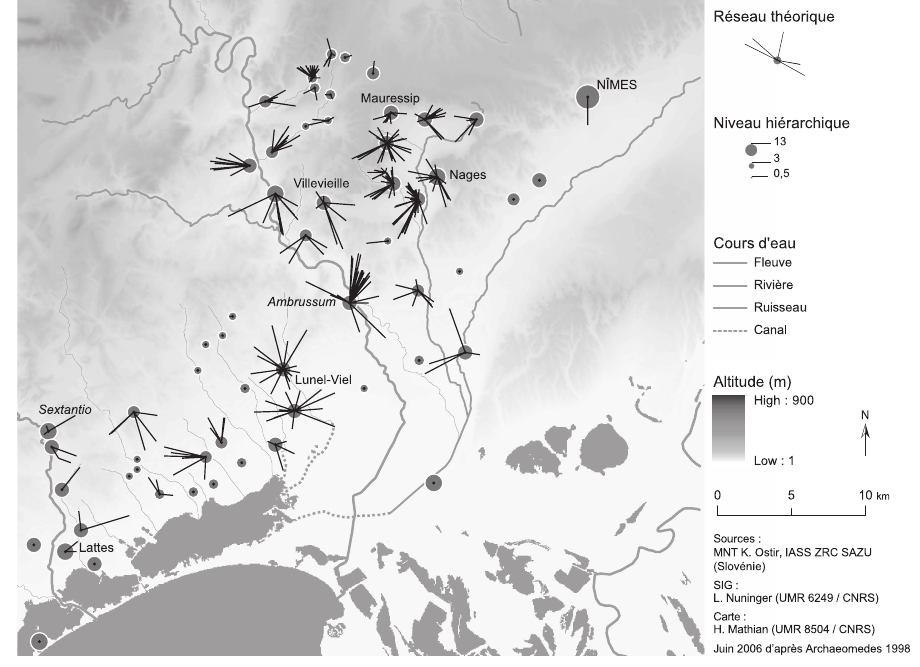
\includegraphics[height=3cm]{images/hierarchi.png}
	\hfil \includegraphics[height=3cm]{images/hierarchyTime.png}
    \end{center}
    
\end{frame}

\begin{frame}{Montreal: NIPS 2015, network workshop}
 Hanna Wallach : ``Computational Social Sciences'':\\

 \begin{itemize}
     \item Latent Network :
	 \begin{center}
	     \includegraphics[height=2.5cm]{images/mailnet.png}
	 \end{center}
     \item Dyadic event analysis : ``country A did action U to country C''\\
	 \begin{itemize}
	     \item extract groups of ``actors'' and type of group of actors interacting with other groups of ``receptors'' with different kind of ``receptors'' and different relation between different groups of actors/receptors.
	     \item reconstruct and analyse geopolitical history
	   
	 \end{itemize}
     \item Bayesian latent variable models: $P(Y,\Omega | X,H)$
 \end{itemize}


    
\end{frame}

\begin{frame}{Montreal: Mc Gill}
    Georgres Grantham: Retired researcher from the good old ``cliometrics''time who recently wrote:
    \begin{quote}
	G. Grantham, A Search-Equilibrium Approach to the Roman Economy. Latomus \& Peeters, 2015.
    \end{quote}
    in :
    \begin{quote}
	K. Verboven and P. Erdkamp, Structure and performance in the Roman economy: models, methods and case studies. Latomus \& Peeters, 2015.
    \end{quote}


    \begin{itemize}
	\item Really interested in the project and found the article going in the right direction \dots
    \item Cities as proxy for economical development 
    \item Clermont-Ferrand studies of hierarchy between villae using photos
    \end{itemize}
    \includegraphics[height=3cm]{images/clermont.png}

    
\end{frame}
\begin{frame}
   \begin{center}
       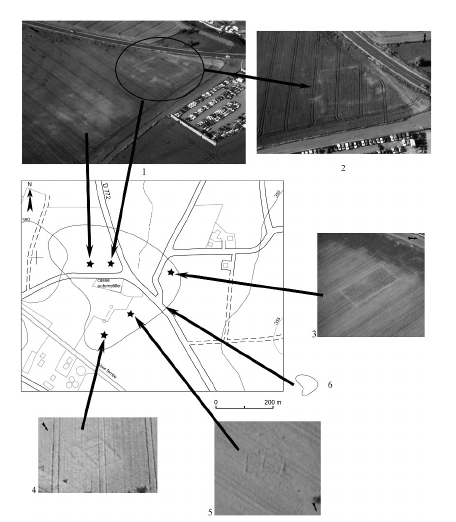
\includegraphics[width=\textwidth]{images/clermontPhoto.png}
   \end{center}
\end{frame}

\begin{frame}{Montreal: UdeM}
Frederic Bouchard : Philosopher of Biology, Chair of Phylosophy, Vice rector of UdeM.
    \begin{itemize}
	\item draft of the MS7 Abstract.
	\item Jean François Gauvin ( Chaire de recherche du Canada sur les transformations de la communication savante) \&   Pr. Vincent Larivière (director of the Collection of Historical Scientific Instruments (CHSI) @ Harvard Semitic Museum) :\\
	    use epigraphic data from Semitic museum to study cultural (scientific ) evolution.
    \end{itemize}

    
\end{frame}

\begin{frame}{Montreal: UQAM}

    10 minutes talk in ``L'oeuf ou la poule''( the egg or the chicken?) about ``Model in science''
    \begin{center}
	\includegraphics[width=.8\textwidth]{images/lolp.png}
    \end{center}

\end{frame}

\begin{frame}{MS7}
    Conference ``Models \& Simulations'' in Barcelona May 18th-20th, 2016\\
    \begin{itemize}
	\item deadline abstract the 22 December,
	    \vfil
	\item submitted with Ale and Bernardo (and Remesal)
	    \vfil
	\item answer in february
	    \vfil
    \end{itemize}
\end{frame}

\begin{frame}{Actual Work}
    \begin{itemize}
	\item Manchester DACAS bursary: Data and Cities as Complex Adaptive Systems, by the Manchester Metropolitan University,Manchester School of Architecture.
	    \vfil
	\item Sante Fe Summer School: 2 pages statements of reacher interest (deadline tomorrow)
	    \vfil
	\item JIPI, The 2nd of February (cf María)\\
	    \begin{center}
		
\includegraphics[height=4cm]{images/jipi.png}
	    \end{center}
	\item Dijon CompleNet
    \end{itemize}
    
\end{frame}

\begin{frame}{CompleNet 2016}
    \begin{center}
	\begin{columns}
	    \begin{column}{.5\textwidth}
		\begin{center}
		    Small-World
		\end{center}
		\begin{column}{.2\textwidth}
			\tiny
			200 Nodes,\\ 
			400 Edges,\\
			Density:.02
		\end{column}
		\begin{column}{.8\textwidth}
		    \begin{figure}
			\includegraphics[width=\textwidth]{images/graphSW.png}
		    \end{figure}
		\end{column}
		\begin{center}
		    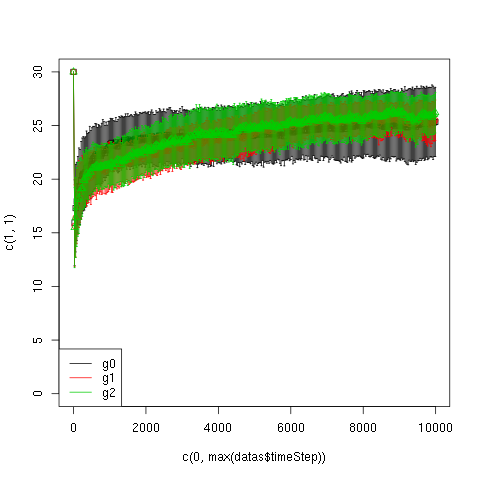
\includegraphics[width=.6\textwidth]{images/scoreSW.png}
		\end{center}
	    \end{column}
	    \begin{column}{.5\textwidth}
		\begin{center}
		    Scale Free
		\end{center}
		\begin{column}{.2\textwidth}
			\tiny
			200 Nodes,\\
			396 Edges,\\
			Density:.02
		\end{column}
		\begin{column}{.8\textwidth}
		    \begin{figure}
			\includegraphics[width=\textwidth]{images/graphSF.png}
		    \end{figure}
		\end{column}
		\begin{center}
		    \includegraphics[width=.6\textwidth]{images/scoreSF.png}
		\end{center}

	    \end{column}
	\end{columns}
    \end{center}
\end{frame}
\begin{frame}{CompleNet 2016}
    Cultural dynamics can lead efficient decentralized market \textbf{when cultural network exhibit certain essential properties}
    
\end{frame}

\end{document}

